\Chapter{Literature Review}

\section{Suggested Approach}

As with suggestions provided concerning the Introduction, in which a funnel type of approach was suggested, essentially going from broader issues to more specific ones, a similar approach can be highly effective for the literature review. A literature review is one of the most difficult chapters to write, and particularly when it comes to deciding what should -- and should not -- be provided. Often students provide too much, and go into an excessive amount of detail, on things covered in the literature review. A guiding principle is demonstrating your awareness of the field and related works that are (or could) guide your work, are important to consider (eg. standards) or that you are building upon. You do not really want to have a literature review that are essentially recreating lecture notes or summaries on the theory; certainly in some case you do need brief recaps of techniques or theories (especially with references to direct the reader to resources where they can touch up on their understanding of the issues covered) -- MSc student in particularly are likely going to need advice from their supervisor in making an effective choice of what should be, and should not be, recapped in the literature review.

The Figure \ref{fig:litreviewfunnel} provides an illustration of a suggested "funnel structure" around which you could build your literature review. This structure should work for either BSc, MSc or PhD and the difference between them (e.g. BSc towards PhD) is the scale, scope, complexity and novelty of these. For example, a BSc will be small scale (often just a very specific gap in knowledge, if any; it might be more a build and test rather than a finding something to fill a knowledge gap) and not so complex and might not even have any novelty. A MSc would be a bit larger in scale (but not too much), more complex (likely more things happening and more complicated connections between these) and hopefully (but not necessarily) having some novelty (for a MSc it could just be using a different platform e.g. a Raspberry Pi instead of an Arduino to trial an embedded solution). A PhD is of course quite a step up from a MSc in terms of scope, complexity, and certainly is needed to be proven a novel contribution in that it has added new knowledge (i.e. filled a non-trivial gap in the research literature).

The parts of the literature review funnel structure are explained briefly in the points below. Note that you do not really want to just use these bullet points for the names of the subheadings of you lit review, you need to think a bit more about what would be suitable heading names and sequencing of these. These tips are only suggestions to help you think about how to construct you literature review and should not be considered a prescribed structure or method to use (theses do tend to be quite unique, there is not really one method that would works for all cases, generally it is built through a process of reviewing what others have done, writing and reworking the document).

\begin{figure}
	\centering
	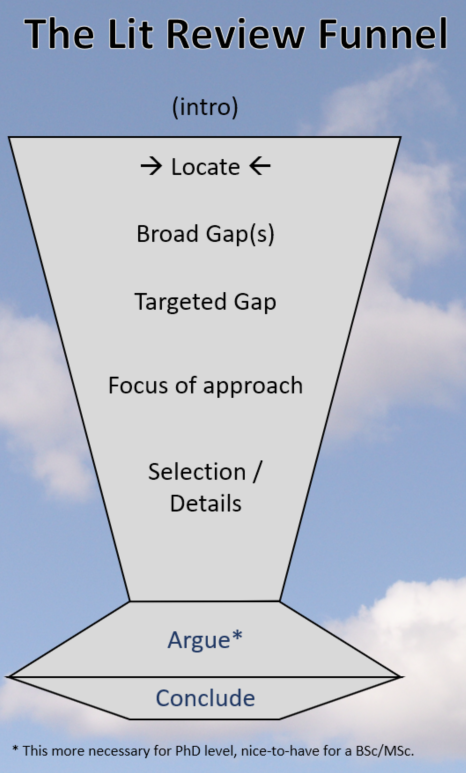
\includegraphics[width=0.7\linewidth]{Chapters/Figures/litreview_funnel}
	\caption{Literature review funnel structure}
	\label{fig:litreviewfunnel}
\end{figure}

\begin{itemize}
	\item Intro: Start with explaining how the approach to the lit review and its structure.
	\item Locate: Entry to the top funnel, outlining what you will cover. Start drilling down, the field, broad theories. Cover significant aspects of main thinking/trends you are plugging in to.
	\item Gap(s): Ideally bring the discussion towards a point that you identify gaps in research or areas that need further investigation.
	\item Targeted gap: Of the various gaps identified indicate which one(s) you will focus on 
	in this project (for BSc/MSc probably just one gap; PhD may have more but not too many).
	\item Focus of approach Get into the more specific issues, techniques that will be used to solve the problem and review these theories/methods/tools.
	At the same time you may cover a few ‘alternate approaches’ that could inspire your approach or what you are learning from to refine the approach you have chosen, learning from past attempts or similar types of investigation (they obviously don’t need to be trying to do the same thing but some relation/relevance to your project).
	\item Selection / Details: At this part you get into more specifics of potential development tool or library you planning to use and why.
	This can be handled fairly easily, e.g. doing brief literature surveys, e.g. web searches, on what are the most popular tools. Could expanded by describing a methodology to use for selecting these tools, the result of this could be tables showing the tool/library options, their pros and cons*. The tool rated best could be the one to choose in the project.
	\item Argue: Nice-to-haves (emphasising ‘the researcher’ and research benefits) Broaden out with argument, identifying new knowledge needed, how this research investigation will contribute new understanding. This part depends on space availability*.
	\item Conclude/Summary: Definitely, try to close in some elegant way. Could be done with a short summary of key observations/gaps and useful theories/methods you’ll build on. For an e.g. PhD proposal in particular you could end it by justifying (reaffirming the need for) this research.
	\item *: items marked by asterisk are more necessary for PhD level, but still a nice-to-have for a BSc/MSc dissertation.
\end{itemize}

